%\documentclass[11pt,twocolumn]{article}
\documentclass{llncs}
\bibliographystyle{unsrt}
\usepackage{graphicx,wrapfig,lipsum}
\usepackage{url}
\usepackage{hyperref}
\usepackage{subcaption}         % include subfigure
\usepackage{booktabs}
\usepackage{array}
\bibliographystyle{splncs03}

\begin{document}

\title{Early evaluation of the hybrid cluster with torus interconnect aimed at cost-effective molecular-dynamics simulations}

\author{%
Vladimir~V.~Stegailov\inst{1},
Alexander~Agarkov\inst{2},
Sergey~Biryukov\inst{2},
Timur~Ismagilov\inst{2},
Nikolay~Kondratyuk\inst{1}\inst{3}\inst{4},
Evgeny~Kushtanov\inst{2},
Dmitry~Makagon\inst{2},
Anatoly~Mukosey\inst{2},
Alexander~Semenov\inst{2},
Alexey~Simonov\inst{2},
Vyacheslav~Vecher\inst{1}\inst{3}
}
%
\authorrunning{V.~Stegailov et al.} % abbreviated author list (for running head)
%
\institute{Joint Institute for High Temperatures of RAS, Moscow, Russia\\
\and NICEVT, Moscow, Russia\\
\and Moscow Institute of Physics and Technology, Dolgoprudny, Russia\\
\and National Research University Higher School of Economics, Moscow, Russia
%FIXME Владимир, может быть, не очень хорошо здесь указывать почту из ВШЭ?
\email{v.stegailov@hse.ru}
}

\maketitle

\begin{abstract}
In this paper, we describe the Desmos cluster that consists of 32 hybrid nodes connected by a low-latency high-bandwidth torus interconnect. This cluster is aimed at cost-effective classical molecular dynamics calculations. We present strong scaling benchmarks for GROMACS and LAMMPS and compare the results with other HPC systems. This cluster serves as a test bed for the Angara interconnect and verifies its ability to unite MPP systems speeding-up effectively MPI-based applications. The interconnect is based on the Angara NIC that supports 3D and 4D torus network topologies. We describe the interconnect presenting typical MPI benchmarks.  
\end{abstract}


\section{Introduction}

Rapid development of parallel computational methods and supercomputer hardware provide great benefits for atomistic simulation methods. At the moment, these mathematical models and computational codes are not only the tools of fundamental research but the more and more intensively used instruments for diverse applied problems~\cite{Heinecke-etal-MD-Book-2015}. For classical molecular dynamics (MD) the limits of the system size and the simulated time are trillions of atoms~\cite{MD-on-SuperMUC-2013} and milliseconds~\cite{Piana-Klepeis-Shaw-2014} (i.e. $10^9$ steps with a typical MD step of 1~femtosecond).

There are two mainstream ways of MD acceleration. The first one is the use of distributed memory massively-parallel programming (MPP) systems. For MD calculations, domain decomposition is a natural technique to distribute both the computational load and the data across nodes of MPP systems~\cite{Sutmann2002}. Corresponding load-balancing problems can be usually solved very efficiently (e.g.~\cite{BegauSutmann-2015}).

The second possibility consists in the increase of the computing capabilities of individual nodes of MPP systems. Multi-CPU and multi-core shared-memory node architectures provide essential acceleration. However, the scalability of shared memory systems is limited by their cost and speed limitations of DRAM access for multi-socket and/or multi-core nodes. It is the development of GPGPU technologies that boosts significantly the performance of shared-memory systems.

This year is the 10th anniversary of Nvidia CUDA technology that was introduced in 2007 and provided a convenient technique for GPU programming. Many computational algorithms have been rewritten and thoroughly optimized to use the GPU capabilities. However, the majority of them deploy only a fraction of the GPU theoretical performance even after careful tuning, e.g. see~\cite{StegailovSmirnov-MatModCompSim2016,StegailovOrekhovSmirnov-PaCT2015,Wyrzykowski-3DMPDATAtoGPU-adaptation-2016}. The sustained performance is usually limited by the memory-bound nature of the algorithms.

Among GPU-aware MD software one can point out GROMACS~\cite{Berendsen199543} as, perhaps, the most computationally efficient MD tool and LAMMPS~\cite{LAMMPS1995} as one of the most versatile and flexible for MD models creation. Different GPU off-loading schemes were implemented in LAMMPS~\cite{Trott-etal-USER-CUDA-2010,Brown-etal-lammpsGPU-2011,Brown-etal-lammpsGPU-2012,CarterEdwards2014}. GROMACS provides a highly optimized GPU-scheme as well~\cite{Abraham201519}.

There are other ways to increase performance of individual nodes: using GPU accelerators with OpenCL, using Intel Xeon Phi accelerators or even using custom built chips like MDGRAPE~\cite{Ohmura20130387} or ANTON~\cite{Piana-Klepeis-Shaw-2014}. Currently, however, general purpose Nvidia GPUs provide the most cost-effective way for high performance MD calculations~\cite{Kutzner2015}. 

Modern MPP systems can unite up to $10^5$ nodes for solving one computational problem. For this purpose, MPI is the most widely used programming model. The architecture of the individual nodes can differ significantly and is usually selected (co-designed) for the main type of MPP system deployment. The most important component of MPP systems is the interconnect that properties stand behind the scalability of any MPI-based parallel algorithm.

In this work, we describe the Desmos computing cluster that is based on cheap 1CPU+1GPU nodes connected by an original Angara interconnect with torus topology. We describe this novel interconnect and the resulting performance of the cluster for MD models implemented in GROMACS and LAMMPS.


\section{Related work}

Torus topologies of the interconnect has several attractive aspects in comparison with fat-tree topologies. In 1990s, the development of MPP systems has its peak during the remarkable success of Cray T3E systems based on the 3D torus interconnect topology~\cite{Scott96thecray}. Cray T3E was the first supercomputer that provided 1~TFlops of sustained performance. In June 1998 Cray T3E occupied 4 of top-5 records of the Top500 list. In 2004, after several years of the dominance of Beowulf clusters, a custom-built torus interconnect appeared in the IBM BlueGene/L supercomputer~\cite{Adiga:2005:BGT:1665957.1665963}. Subsequent supercomputers of Cray and IBM had torus interconnects as well (with the exception of the latest Cray XC series). Fujitsu designed K~Computer based on the Tofu torus interconnect~\cite{Tofu-Interconnect-2012}. The AURORA Booster and GREEN ICE Booster supercomputers are based on the EXTOLL torus interconnect~\cite{Extoll-2015}.

\begin{wrapfigure}{r}{5.5cm}
%\centering
%\includegraphics[width=0.5\textwidth]{img/desmos_backpanel.pdf}
\includegraphics[width=5.5cm]{img/desmos_backpanel.pdf}
\caption{The Desmos cluster.}
\end{wrapfigure}

Among the references to the recent developments of original types of supercomputer interconnects in Russia, we can mention the MVS-Express interconnect based on the PCI-Express bus~\cite{EliGorLev12}, the FPGA prototypes of the SKIF-Aurora~\cite{AdaKliKli10} and Pautina~\cite{KliShvKhr15} torus interconnects. Up to this moment the Angara interconnect has been evolving all the way from the FPGA prototype~\cite{KorMakBor10,MukSemSim15} to the ASIC-based card~\cite{AgIsmMakSemSim16}. 

MD benchmarks are among the most popular tests for supercomputers. For example, ApoA1 (protein in water) is a widespread model and we can find the corresponding benchmark data for Cray XK6~\cite{NAMD-CrayXK6-2012}, for IBM BlueGene/P and BlueGene/Q systems~\cite{NAMD-BlueGene-2013}, for K Computer~\cite{NAMD-KComputer} (in all cases calculations were made with NAMD). The AURORA Booster supercomputer was benchmarked using LAMMPS~\cite{Extoll-2015}.

There are examples of the development of alternative highly optimized MD codes for supercomputers. The MD code ls1~mardyn was optimized for Intel x86 CPUs including vectorization and shared-memory parallelization that allowed to simulate the multi-trillion atoms Lennard-Jones liquid model on 146016 cores of the SuperMUC supercomputer~\cite{MD-on-SuperMUC-2013}. 
%A special MD code MODYLAS was developed for K~Computer and allowed to perform the 100 ns-long MD calculation of 10 million-atom system within 3 days (5 ms/step)~\cite{MODYLAS-2013}.

Torus topology is believed to be beneficial for strong scaling of many parallel algorithms. However, the accurate data that verify this assumption are quite rare. Probably, the most extensive work was done by Fabiano Corsetti who compared torus and fat tree topologies using the SIESTA electronic structure code and six large-scale supercomputers belonging to the PRACE Tier-0
network~\cite{Corsetti2014}. The author concluded that machines implementing torus topologies demonstrated a better scalability to large system sizes than those implementing fat tree topologies. The comparison of the benchmark data for CP2k showed a similar trend~\cite{StegailovOrekhovSmirnov-PaCT2015}.


\section{The Desmos Cluster}

The hardware for the cluster was selected in order to maximize (within the budget limit) the number of nodes and the efficiency of a single node for MD workloads. The resulting node configuration is shown in Table~\ref{tab:node}.

The Nvidia GeForce 1070 cards have no error-correcting code (ECC) memory in contrast to professional accelerators. For this reason, it was necessary to make sure that there is no hardware memory errors in each GPU. Testing of each GPU was performed using MemtestG80~\cite{Haque:2010:HDS:1844765.1845231} during more than 4 hours for each card. No errors were detected for 32 cards considered.

The cooling of the GPU cards was a special question. We used ASUS GeForce GTX 1070 8GB Turbo Edition. Each card was partially disassembled prior to installation into 1U chassis. The plastic cover and the dual-ball bearing fan were removed that made the card suitable for horizontal air flow cooling inside chassis.

The nodes are connected by Gigabit Ethernet and Angara interconnect (in the 4D-torus $4\times2\times2\times2$). Due to budget limitations we did not use all possible ports for the full 4D-torus topology. The currently implemented topology is 4D-torus $4\times2\times2\times2$ $(X \times Y \times Z \times K)$ but each node along $Y, Z, K$ dimensions is connected to another node by one link only.

There is a front-end node with the same configuration as all 32 computing nodes of the cluster (the front-end node is connected to GE only). The cluster is running under SLES~11~SP4 with Angara MPI (based on MPICH 3.0.4).

The cluster energy consumption is 6.5~kW in the idle state and 14.4~kW under full load.

\begin{table}[t]
\caption{\label{tab:node}Components of a single node (Moscow prices for October~2016)}
\begin{center}
\renewcommand{\arraystretch}{1}
\centering
\begin{tabular}{ p{20mm} p{65mm} p{20mm} }
\toprule
\textbf{Chassis} & Supermicro SuperServer 1018GR-T & 955 USD \\
\midrule
\textbf{CPU} & Intel Xeon E5-1650v3 (6 cores, 3.5 GHz) & 700 USD \\
\midrule
\textbf{GPU} & Nvidia GeForce GTX 1070 (8 GB GDDR5) & 550 USD \\
\midrule
\textbf{DRAM} & DDR4 8 GB & 70 USD\\
\midrule
\textbf{Storage} & HDD 500 GB & 44 USD\\
\midrule
& Total price & 2319 USD\\
\bottomrule
\end{tabular}
\end{center}
\end{table}


\begin{table}
\caption{\label{tab:systems}Comparison of the Desmos cluster with the Polytekhnik cluster used as a reference for MPI benchmarks}
\begin{center}
\renewcommand{\arraystretch}{1}
\begin{tabular}{ l c c }
\toprule
\textbf{Cluster} & \textbf{Desmos} & \textbf{Polytekhnik} \\
\midrule
\textbf{Chassis} & SuperServer 1018GR-T & RSC Tornado \\
\midrule
\textbf{Processor} & E5-1650v3 (6c, 3.0 GHz) & 2 x E5-2697v3 (14c, 2.6 GHz)\\
\midrule
\textbf{GPU} & Nvidia GeForce GTX 1070& --- \\
\midrule
\textbf{Memory} & DDR4 8 GB & DDR4 64 GB\\
\midrule
\textbf{Number of nodes} & 32 & 612 \\
\midrule
\textbf{Interconnect} & Angara 4D-torus $4\times2\times2\times2$ & Infiniband 4x FDR 2:1\\
\midrule
\textbf{Operating system} & SLES 11 SP4 & CentOS 7.0.1406 \\
\midrule
\textbf{Compiler} & Intel Parallel Studio XE 2017 & Intel Parallel Studio XE 2016 \\
\midrule
\textbf{MPI} & Angara MPI  & Intel MPI 5.1.2 \\
  &  (based on MPICH 3.0.4) &   \\
\bottomrule
\end{tabular}
\end{center}
\end{table}



\section{The Angara Interconnect}

The Angara interconnect is a Russian-designed communication network with torus topology. The interconnect ASIC was developed by JSC NICEVT and manufactured by TSMC with the 65 nm process. 

The Angara architecture uses some principles of IBM Blue Gene L/P and Cray Seastar2/Seastar2+ torus interconnects. The torus interconnect developed by EXTOLL is a similar project~\cite{Extoll-2015}. The Angara chip supports deadlock-free adaptive routing based on bubble flow control~\cite{Puente:1999:ABR:850940.852882}, direction ordered routing~\cite{Scott96thecray,Adiga:2005:BGT:1665957.1665963} and initial and final hops for fault tolerance~\cite{Scott96thecray}.

Each node has a dedicated memory region available for remote access from other nodes (read, write, atomic operations) to support the OpenSHMEM and PGAS languages. Multiple parallel programming models are supported MPI and OpenMP including.

The network adapter is a PCI Express extension card that is connected to the adjacent nodes by up to 6 cables (or up to 8 with an extension card). The following topologies are supported: a ring, 2D, 3D and 4D tori. 

To provide more insights into Angara communication behavior we present a performance evaluation comparison of the Desmos cluster and the Polytekhnik cluster with the Mellanox Infiniband 4x FDR 2:1 blocking interconnect. Table \ref{tab:systems} compares two systems. Both systems are equipped with Haswell CPUs but the processors characteristics differ very much. 

Figure~\ref{fig:latency} shows the latency results obtained by the OSU Micro-Benchmarks test. Angara has extremely low latency 0.85 $\mu$s for the 16 bytes message size and exceeds 4x FDR interconnect for all small message sizes.

We use Intel MPI Benchmarks to evaluate MPI\_Barrier and MPI\_Alltoall operation times for different number of nodes of the Desmos and Polytekhnik clusters. The Angara superiority for small messages explains better results for MPI\_Barrier (Figure~\ref{fig:barrier}) and MPI\_Alltoall with 16 byte messages (Figure~\ref{fig:alltoall_small}). For large messages (256 Kbytes) the Desmos results are worse than that of the Polytechnik cluster (Figure~\ref{fig:alltoall_large}). It can be explained by loose connectivity of the Desmos torus topology (2.5 links per node) and the performance weakness of the current variant of the Angara MPI implementation.

\begin{figure}[th!]
\centering
   \begin{subfigure}{0.45\textwidth}
  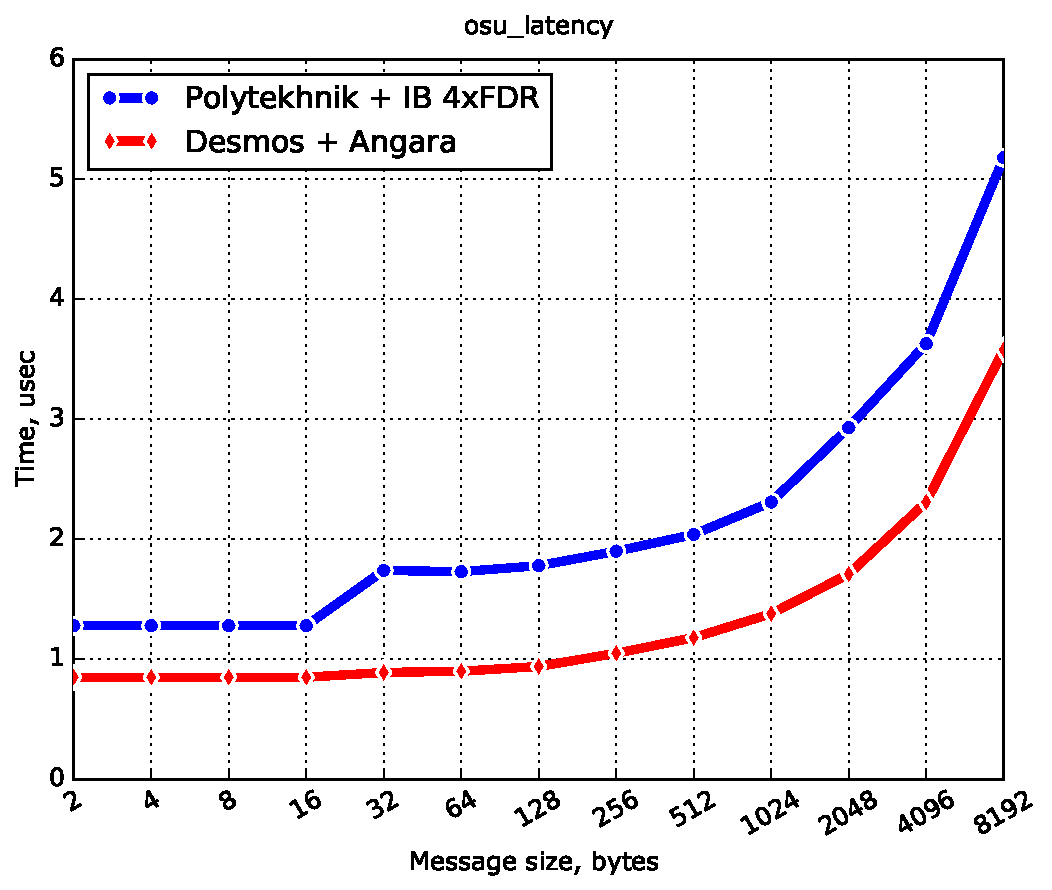
\includegraphics[width=1\textwidth]{img/osu_latency.pdf}\caption{\label{fig:latency}}
  \end{subfigure}
  \begin{subfigure}{0.45\textwidth}
  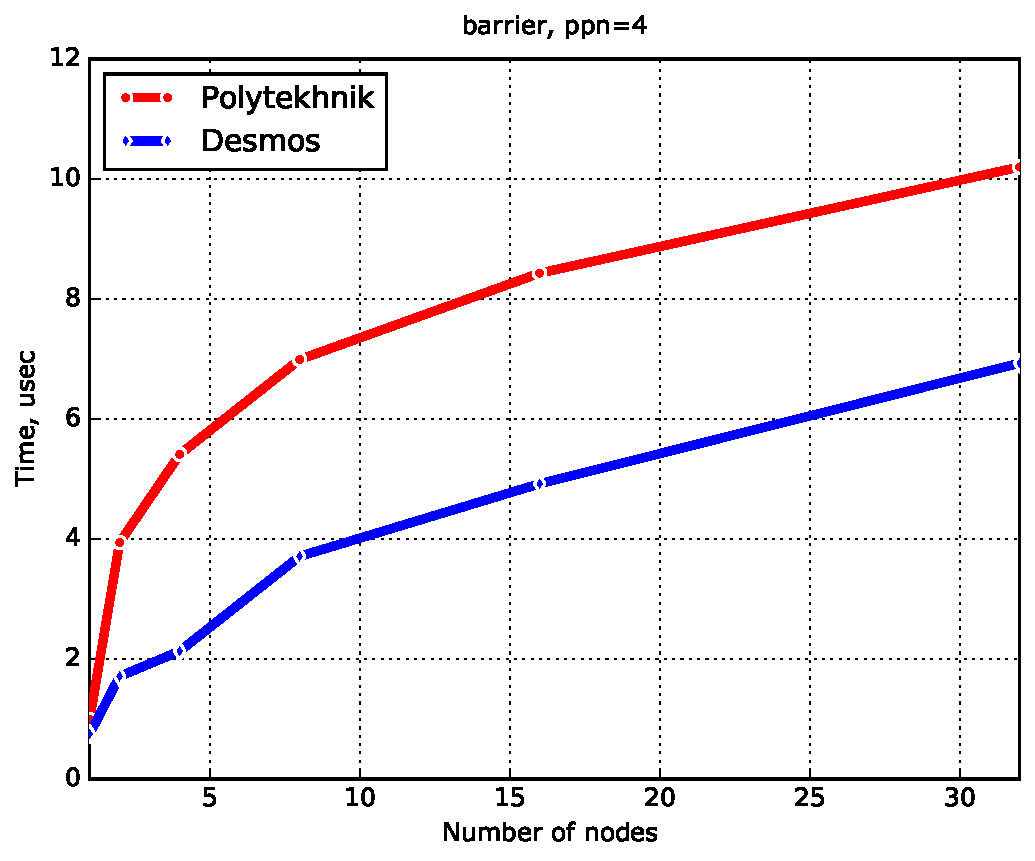
\includegraphics[width=1\textwidth]{img/barrier_ppn4.pdf}\caption{\label{fig:barrier}}
   \end{subfigure}
   \begin{subfigure}{0.45\textwidth}
  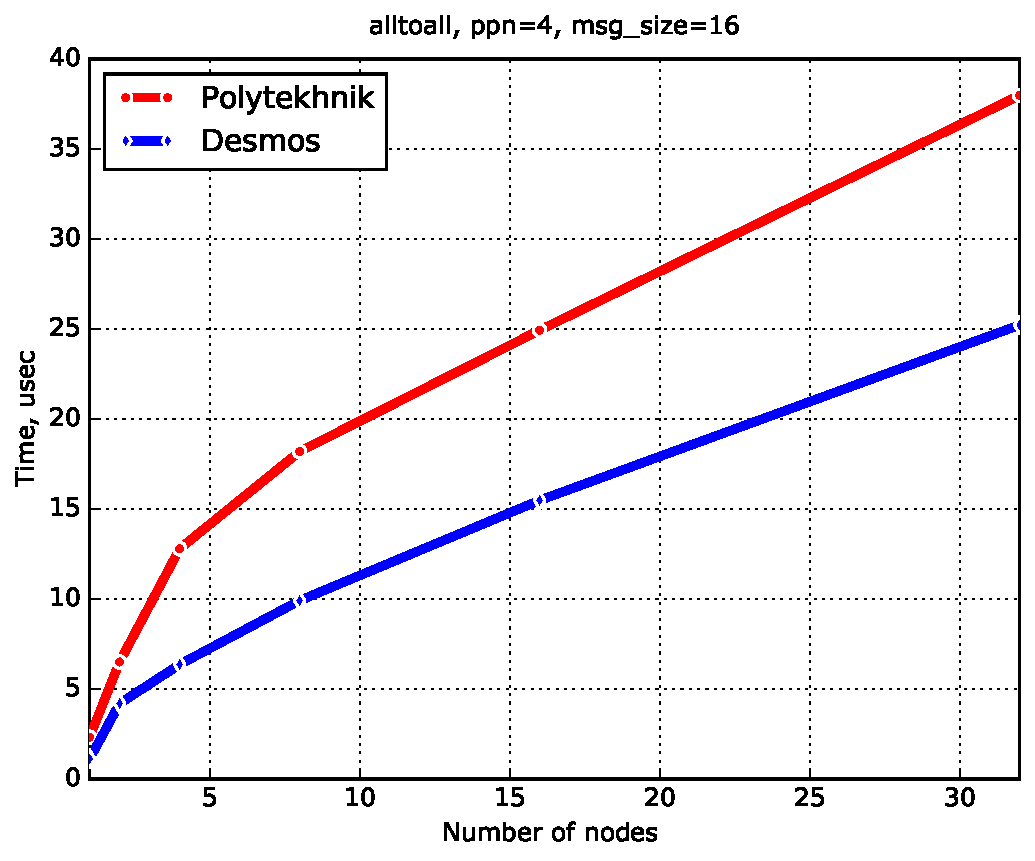
\includegraphics[width=1\textwidth]{img/alltoall_ppn=4_size=16.pdf}\caption{\label{fig:alltoall_small}}
  \end{subfigure}
  \begin{subfigure}{0.45\textwidth}
  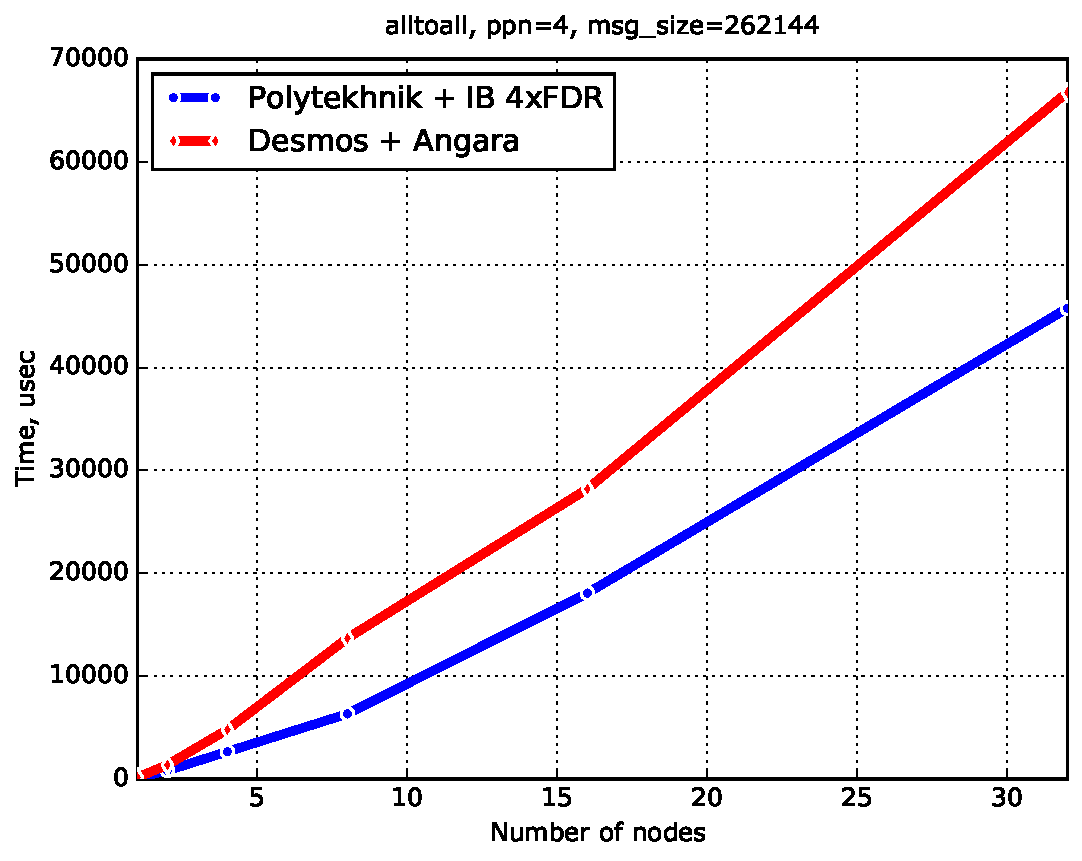
\includegraphics[width=1\textwidth]{img/alltoall_ppn=4_size=262144.pdf}\caption{\label{fig:alltoall_large}}
   \end{subfigure}
\caption{ The OSU latency between two adjacent nodes (a). Times for MPI\_Barrier with 4 processes per node (b). Times for MPI\_Alltoall with 4 processes per node and message sizes 16~b (c) and 256~Kb (d).}
\end{figure}


\section{MD benchmarks}

Nowadays, there is no novelty in the partial use of single precision in MD calculations with consumer-grade GPUs. The results of such projects as Folding@Home confirmed the broad applicability of this approach. Recent developments of optimized MD algorithms include the validation of the single precision solver (e.g.~\cite{Hohnerbach-2016}). In this study we do not consider the questions of accuracy and limit ourselves to the benchmarks of computational efficiency.

The first set of benchmark data is shown on Figure~\ref{c30_lj}. It illustrates the efficiency of LAMMPS, LAMMPS with the GPU package (with mixed precision) or LAMMPS with USER-INTEL package running on one computational node for different numbers of atoms in the MD model. The USER-INTEL package provides SIMD-optimized versions of certain interatomic potentials in LAMMPS. As expected, the CPU+GPU pair shows maximum performance for sufficiently large system sizes. The results for the Desmos node are compared with the results for a two-socket node with 14-core Haswell CPUs (the MVS1P5 cluster). 

We see that for the simple Lennard-Jones (LJ) liquid benchmark the GPU-version of LAMMPS on one Desmos node provides two times higher times-to-solution than the SIMD-optimized LAMMPS on 2 x 14-core Haswell CPUs. However for the liquid C$_{30}$H$_{62}$ oil benchmark the GPU-version of LAMMPS is faster starting from 100 thousand atoms per node.

For comparison, we present the results for the same benchmark on the professional grade Nvidia Tesla K80 card.

\begin{figure}
\centering
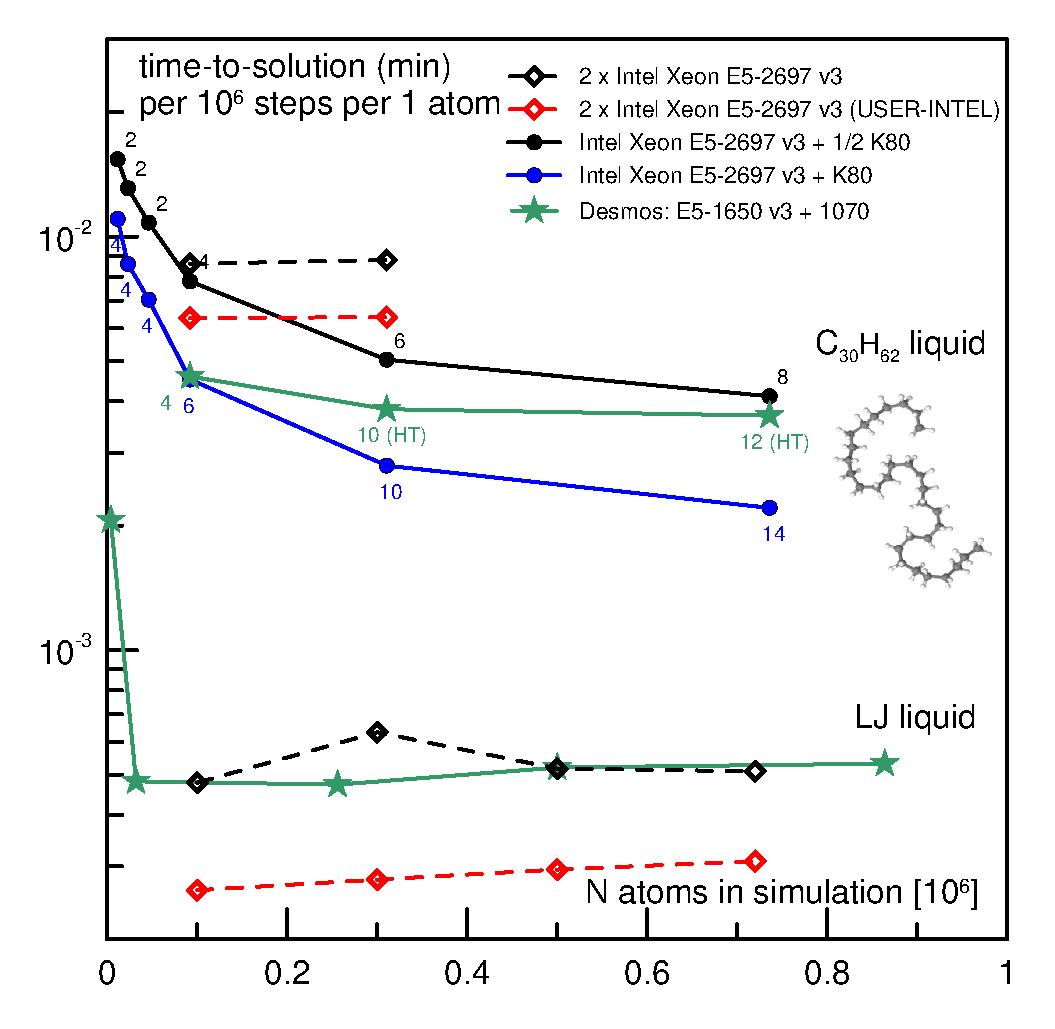
\includegraphics[width=0.7\textwidth]{img/c30_lj.pdf}
\caption{\label{c30_lj} Times-to-solution per atom per timestep for Lennard-Jones liquid and C$_{30}$H$_{62}$ oil LAMMPS MD models of different size and different hardware combinations.}
\end{figure}

An apolipoprotein A1 (ApoA1) in water MD model is a popular benchmark system with $\sim$100k atoms. Figure~\ref{weak_scaling} shows the weak scaling results for the LJ system, for the C$_{30}$H$_{62}$ oil model and for the ApoA1 system. We see that weak scaling becomes better for larger models.

We should mention that weak scaling could be slightly improved after implementation of the topology-aware cartesian MPI-communicators in Angara MPI. 

The ``time-to-solution'' criterion leads us to the evident choice of a time for one MD integration step as one parameter for the metric. The second parameter should characterize the hardware. Usually the number of some abstract processing elements (e.~g. cores) is considered. However although this metric serves well in the \emph{weak} and \emph{strong} scaling benchmarks for the given system, it does not allow to compare essentially different hardware. In order to overcome this problem we consider the total peak performance $R_{peak}$ as a second parameter for the metric that put on equal footing all HPC hardware under consideration~\cite{StegailovOrekhovSmirnov-PaCT2015}.

\begin{wrapfigure}{r}{5.5cm}
%\centering
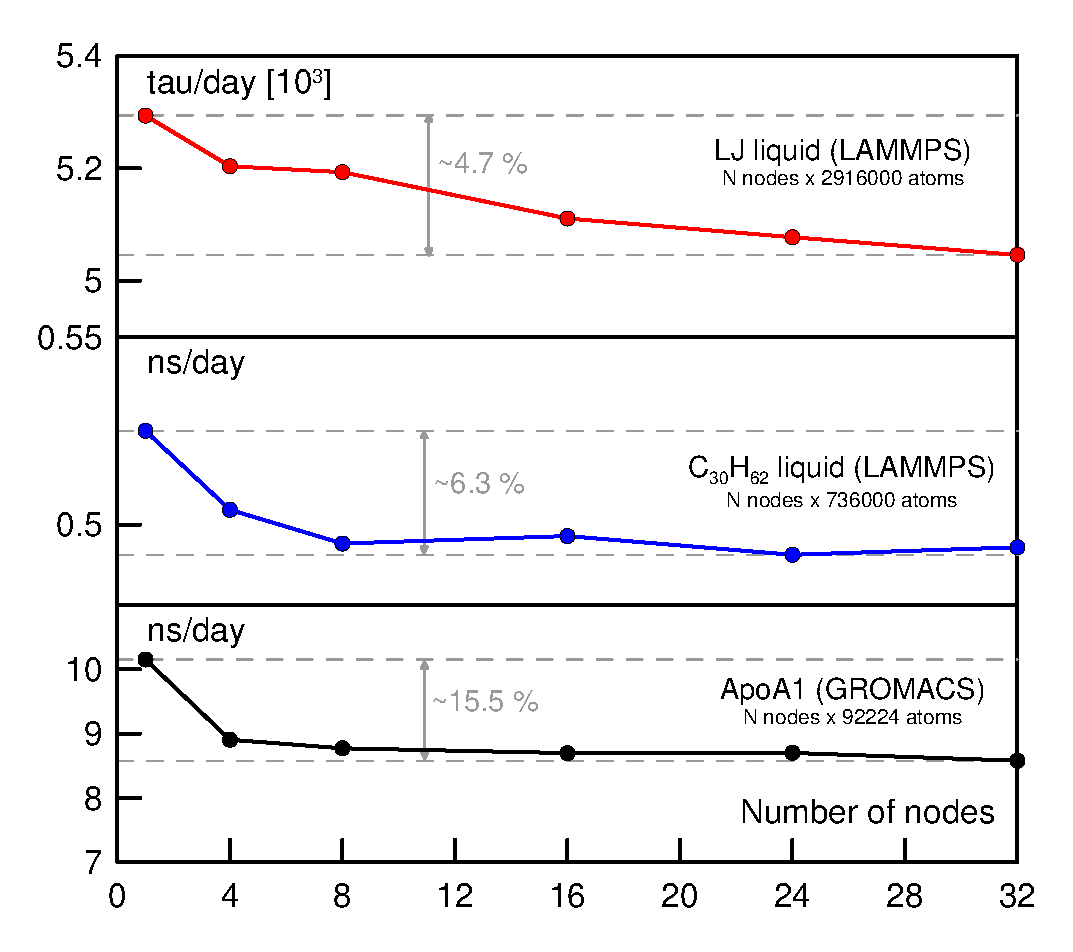
\includegraphics[width=5.5cm]{img/weak_scaling.pdf}
\caption{\label{weak_scaling} Weak scaling benchmarks for the Desmos cluster and three different MD models.}
\end{wrapfigure}

Since the Desmos cluster rely heavily on single-precision performance we need to devise some reasonable conversion of SP Flops to DP Flops. Here we take $R^{node}_{peak} = 6 * 3.5 * 16 + 0.5 * R^{GPU-SP}_{peak} = 336 + 2892 = 3228$~GFlops. 

The performance of different clusters based on ApoA1 test is shown in Figure~\ref{ApoA1} in terms of seconds per 1 atom for 1 MD step and the declared peak performance. The dotted line shows ideal scalability with performance 0.1 MFlops/atom/step.

Despite different architectures and MD software, these data can be used to analyze the efficiency of supercomputer systems for biomolecular MD sudies. The black and green lines with dots show the performance of the CPU cluster with Intel Xeon nodes~\cite{StegailovSmirnov-MatModCompSim2016}. The new Desmos cluster (the purple filled stars) with GROMACS shows better scalability then Cray XK6~\cite{NAMD-CrayXK6-2012} and the K Computer with NAMD. It shows better efficiency than the benchmarks for BlueGene systems\cite{NAMD-BlueGene-2013}. 

The green stars show the 27 times replicated ApoA1 system benchmark for the Desmos cluster. These data show the continuous scaling with larger number atoms per node. It indicates the possibility for adding more nodes to Desmos without noticeable efficiency degradation.

\begin{figure}
\centering
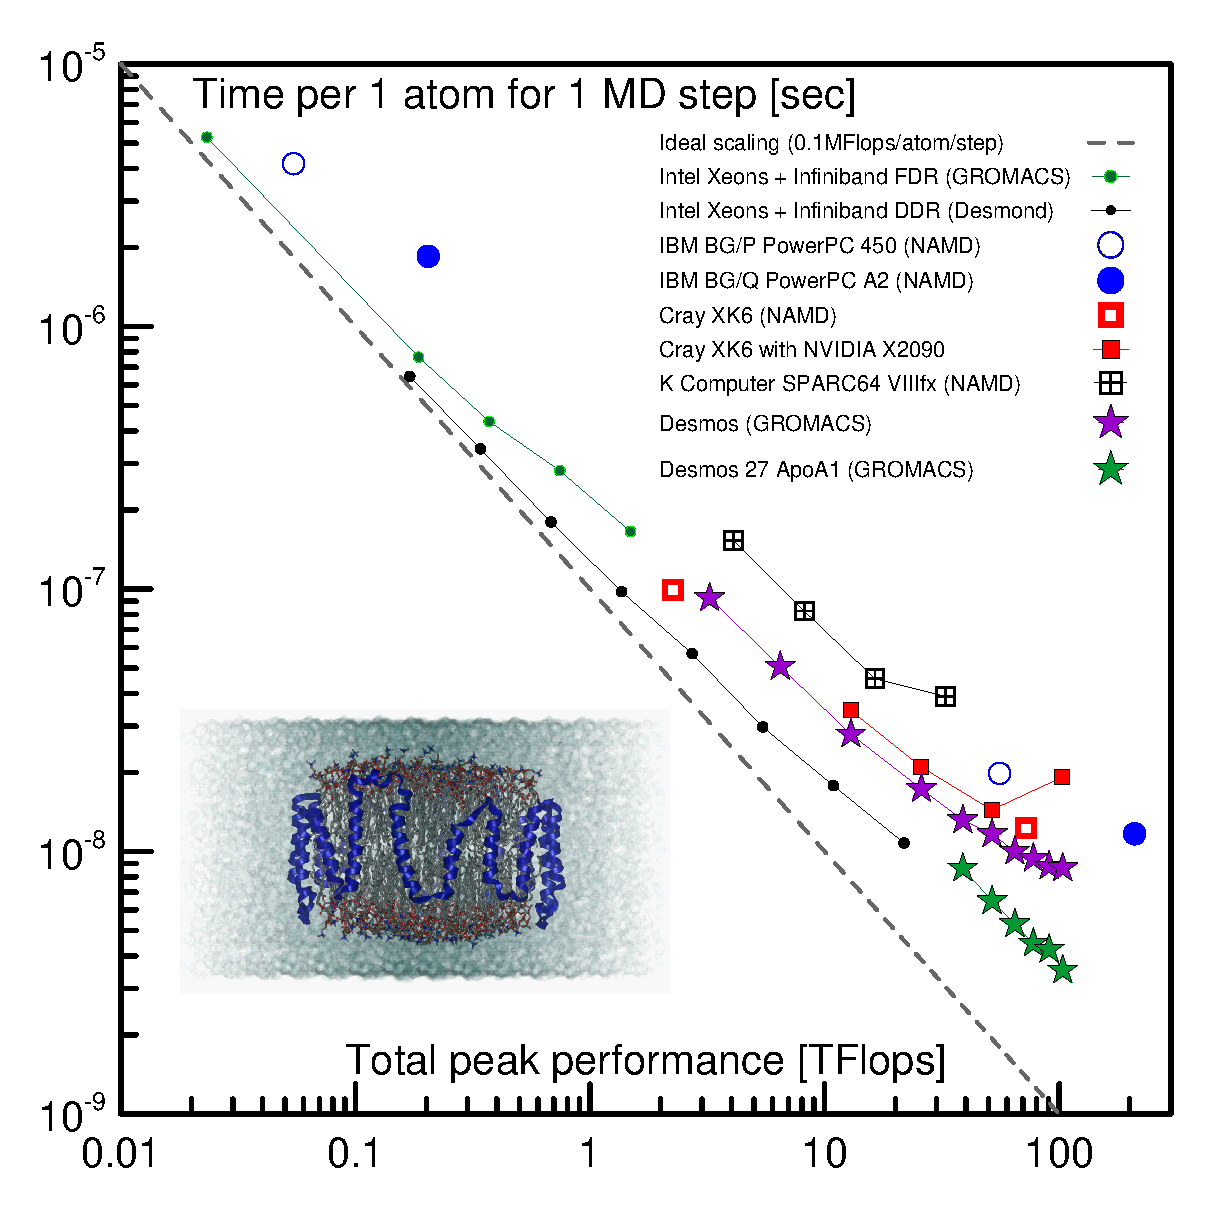
\includegraphics[width=0.6\textwidth]{img/compar_comp.pdf}
\caption{\label{ApoA1} ApoA1 benchmark results obtained with GROMACS for the Desmos cluster (including the 3x3x3 replicated model). For comparison we show the data for the same benchmark but obtained with NAMD for different supercomputers: Cray XK6~\cite{NAMD-CrayXK6-2012}, IBM BlueGene/P and BlueGene/Q~\cite{NAMD-BlueGene-2013}, K Computer~\cite{NAMD-KComputer}.}
\end{figure}

The work~\cite{Kutzner2015} gives very instructive guidelines for achieving the best performance for the minimal price in 2015. Authors compared different configurations of clusters using two biological benchmarks: the membrane channel protein embedded in a lipid bilayer surrounded by water (MEM, $\sim $100k atoms) and the bacterial ribosome in water with ions (RIB, $\sim$2M atoms). The GROMACS package was used for all tests. We follow the same protocol but use longer MD simulations than in~\cite{Kutzner2015} to obtain the best performance.

\begin{figure}
\centering
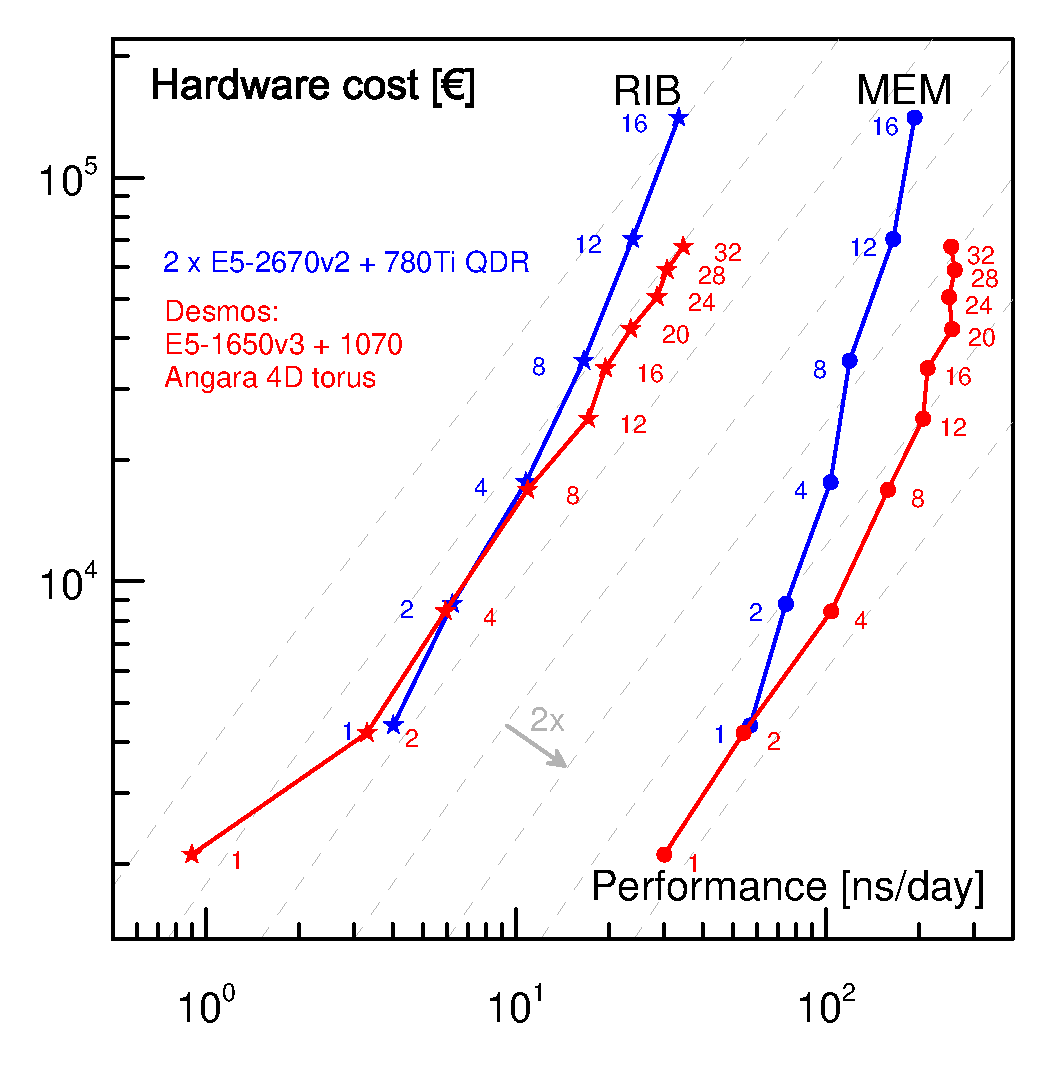
\includegraphics[width=0.6\textwidth]{img/best_bang.pdf}
\caption{\label{BestBang} The cost of hardware vs achieved performance for MEM and RIB benchmarks. The dashed lines show ideal scaling. Desmos results are compared with the published results~\cite{Kutzner2015}.}
\end{figure}

We compare the results obtained on Desmos cluster with the best choice of~\cite{Kutzner2015}: the nodes that consist of 2 socket Xeon E5-2670 v2 with 2 780Ti and connected via InfiniBand QDR. The costs of hardware in Euros are displayed on Y axis (for price conversion we use the ratio Euro/USD=1.1 for October 2016) and the performance in ns/day is shown on X axis in Figure~\ref{BestBang}. The numbers show the number of nodes used. The grey lines indicate ideal scaling.

Desmos (red color) shows better strong scaling for the MEM benchmark than the best system configuration provided by Kutzner et al. (blue color)~\cite{Kutzner2015}. The major reason is, of course, the new Pascal GPU architecture. The saturation is achieved after 20 nodes which corresponds to the small amount of atoms per node, below the GPU efficiency threshold. In the case of the RIB benchmark, Desmos demonstrates ideal scaling after 16 nodes which shows that the productivity can be increased with larger number of nodes.


\section{Conclusions}

In the paper we described the cost-effective Desmos cluster targeted to MD calculations. The results of this work confirmed the high efficiency of commodity GPU hardware for MD simulations. The Desmos cluster is the first application of the Angara interconnect for a GPU-based MPP system. The features of the Angara interconnect provided very reasonable level of efficiency for the MPP system considered. The MPI benchmarks presented supported the competitive level of this network for HPC applications.

The results of the work were obtained using computational resources of Peter the Great Saint-Petersburg Polytechnic University Supercomputing Center (\url{http://www.spbstu.ru}). The authors are grateful to the Forsite company for the access to the server with Nvidia Tesla K80. The authors acknowledge Joint Supercomputer Centre of Russin Academy of Sciences (\url{http://www.jscc.ru}) for the access to the MVS-10P supercomputer.

The work of the JIHT team (V.S., N.K. and V.V.) was supported by the grant No.\,14-50-00124 of the Russian Science Foundation. Their work included the development of the Desmos cluster architecture, tuning of the MD codes performance and MD benchmarks. The NICEVT team developed the Angara interconnect and the corresponding low-level software stack, built and tuned the Desmos cluster.

\textbf{\textit{Comment for reviewers}}. Unfortunately, the Angara interconnect bandwidth is the subject of the non-disclosure agreement of the Angara project.

\bibliography{references,references_MD}

\end{document}
